\hspace{24pt}
In this chapter, we will introduce the method we added to EAGLE to reduce reference bias; explain in detail how we create our hypothetical sequence based on the variant and how to quickly search through an FM-index to obtain those missing reads, and finally add these reads to the pileup that EAGLE considers.
\section{Overview}
The red area in Figure~\ref{core-workflow} shows our implementation of the core workflow of reducing reference bias on EAGLE, and the whole Figure \ref{core-workflow} is our complete workflow after combining EAGLE. 
We can roughly divide our workflow into the following five parts:

\begin{enumerate}
\item Combine variant information in a VCF file and the reference genome to create a hypothetical sequence which includes individual differences.
\item Build a \textit{read-index}, an FM-index of the read sequences.
\item Use BWA and the read-index to find the reads that match the variant, and then check if they already exists in the pileup.
\item For any reads not found in the pileup, create that read's alignment information mapped against reference sequences 
\item Add read and alignment information to the pileup, to improve the EAGLE calculation.
\end{enumerate}

\begin{figure}[H]
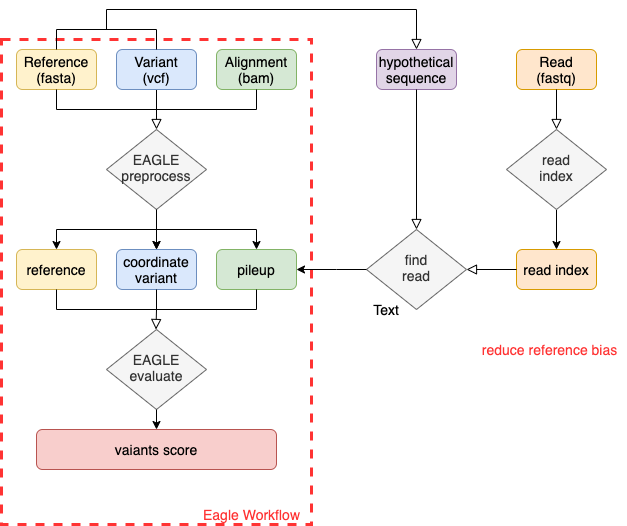
\includegraphics[width=0.8\columnwidth]{body/image/core-workflow.png}
\caption[Core workflow]{The core workflow of EAGLE after adding reference bias reduction.}
\label{core-workflow}
\end{figure}

\section{Hypothetical Sequence}
To reduce the impact of reference bias, the first step we need to construct a hypothetical sequence. Before constructing hypothetical sequence we need variation data and a reference genome. VCF is the standard file format for storing variation data, used by most variant callers (Figure \ref{VCF-format}). FASTA is reference genome format (Figure \ref{FASTA-format}), and it is a text-based format for representing either nucleotide sequences or peptide sequences.

\begin{figure}[H]
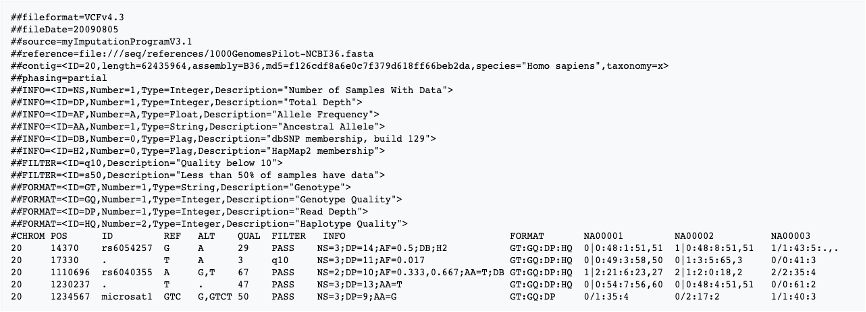
\includegraphics[width=1\columnwidth]{body/image/VCF-format.png}
\caption[VCF format]{Example for VCF format.}
\label{VCF-format}
\end{figure}

\begin{figure}[H]
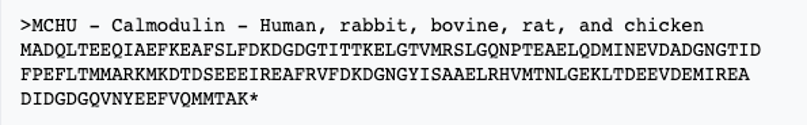
\includegraphics[width=1\columnwidth]{body/image/FASTA-format.png}
\caption[FASTA format]{Example for FASTA format.}
\label{FASTA-format}
\end{figure}

One of the reasons for reference bias is that the reference genome cannot contain individual differences. And our hypothetical sequence is a sequence that combines reference genome and variant. Because we simulate the occurrence of mutation of the reference sequence by combining variant, it includes individual differences. Thus, bases on the information of each variant in the VCF file, including variant position (POS), chromosome name (CHROM), sequence before mutation (REF), and sequence after mutation (ALT), we generate a hypothetical sequence. 

For each hypothetical sequence, according to the variant position, we replace sequence before mutation (REF) to sequence after mutation (ALT). At the same time we will extract the reference genome part front and back in this region, and the length will be the length of a read. The length of this area is long enough to get all the reads we are interested in and also includes individual differences. Figure~\ref{construct-hyposeq} illustrates in detail how we generate a hypothetical sequence based on different types of variants.

We hope to find a read that matches our hypothetical sequence in the FASTQ file to achieve the effect of reducing the reference bias.

\begin{figure}[H]
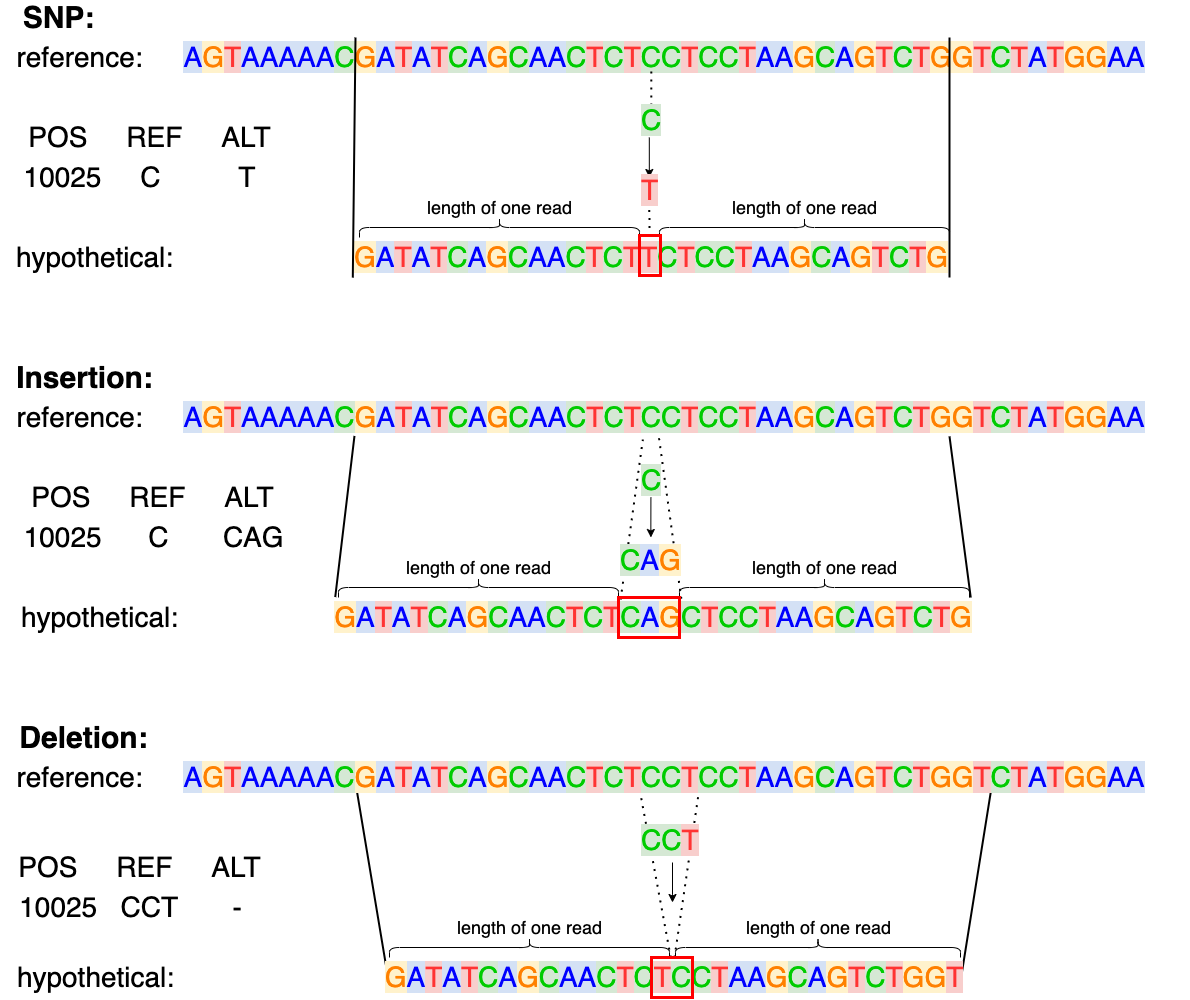
\includegraphics[width=1\columnwidth]{body/image/construct-hyposeq.png}
\caption[construct hypothetical sequence]{Three different cases to construct hypothetical sequence.}
\label{construct-hyposeq}
\end{figure}

\section{Read-index}

Following is an important step for us to find the read that matches our hypothetical sequence. However, if we simply search for matching reads in the FASTQ file, it will cost us a lot of time. 

First we describe general practice: the supposed genome sequence is the reference genome, and we need to map reads on this, just like alignment. Therefore we need to construct index for each hypothetical sequence and then query all the read in FASTQ file. As we mentioned above, we need $O(n\log n)$  ($n$ is reference sequence length) to construct BWT index, and querying will cost $O(\ell)$ ($\ell$ is read length) for each read.

In general situation, the time spent to build an index and perform queries is:
%%
\begin{equation*}
O(n \log n) + O(\ell)
\end{equation*}

It is indeed a very efficient method for standard applications. It only needs to query once for each read, because all reads only need to be aligned to one reference genome sequence. But in our situation, our hypothetical genome sequence is not constant. For each variant we will establish a hypothetical sequence, so if we follow the traditional method, we need to search all the reads every time. Our speed will be very slow.

What would the situation will be if we construct index for read and used our hypothetical sequence to query?
%%
\begin{enumerate}
\itemsep=0em
\item We just need to build index once a time.
\item For each hypothetical sequence, our query will be very fast.
\end{enumerate}


\noindent Let's take an example and some assumptions:


In general situations, we need to create an index for each hypothetical sequence and do a complete read search. It will take time:
\begin{equation*}
\mathlarger{\sum_{h\in H}} \Big\{ \text{build index on } h + \sum_{r\in R}\text{query}~r~\text{on that index} \Big\}
\end{equation*}
where $H$ denotes the set of hypothetical sequences (one for each variant) and $R$ denotes the set of reads.

\begin{flushleft}
Since the hypothetical sequences are very short compared to the combined length of all reads, the time spent on index building can be ignored.  Query time is linear in the total length of the queries so the time needed is approximately:
\begin{equation*}
\mathlarger{\sum_{h\in H}} \Big\{ \sum_{r\in R}\text{query}~r~\text{on index} \Big\} = |H| \times \ell\,|R|
\end{equation*}
Where $|H|$ denotes the number of hypothetical sequences, $\ell$ the read length, and $|R|$ the number of reads.

On the other hand, when building an index on the reads instead of the hypothetical sequences

And through our way of creating a read index, the time would be:
\begin{equation*}
\text{build index on } R + \sum_{h\in H} \text{query}~h \; \approx \; \ell\,|R|\; \log( \ell|R| ) + 2 \ell\,|H|
\end{equation*}
Which is much faster.
\end{flushleft}

According to the above results, we decided to index our reads to generate and read-index, which helps us quickly find reads matching and sequence. Before indexing, we need to remove some information in read file to convert FASTQ format to FASTA format. This is very simple as we describe in Table \ref{tab:FastaToFastq}, then we can directly call BWA index function to construct read-index.

\begin{table}[ht]
\caption{The difference between FASTQ and FASTA format}
\setlength{\tabcolsep}{1mm}{
\begin{tabular}{|c|l|l|l|}
\hline
\rowcolor{gray} 
\multicolumn{2}{|l|}{\cellcolor{gray} }  & \multicolumn{1}{c|}{\cellcolor{gray} {\color{white} \textbf{Fasta}}} & 
\multicolumn{1}{c|}{\cellcolor{gray} {\color{white} \textbf{Fastq}}}\\
\hline
\rowcolor{lightgray}\cellcolor{gray}& 
Line 1 & description of sequence & @sequence id   \\ 
\cline{2-4} 
\cellcolor{gray}&
Line 2  & sequence & sequence \\
\cline{2-4} 
\rowcolor{lightgray}\cellcolor{gray}&
Line 3  & & +\\ 
\cline{2-4} 
\multirow{-4}{*}{\cellcolor{gray}{\color{white} \textbf{format}}} &
Line 4  & & quality value\\ 
\hline
\rowcolor{lightgray}
\multicolumn{2}{|c|}
{\cellcolor{gray}} & NT\_113878.1 chrom1 & @SEQ\_ID \\
\rowcolor{lightgray}
\multicolumn{2}{|c|}
{\cellcolor{gray}} & GATAGTAGTTGCAGCAGGCTAGCTA & GATAGTAGTTGCAGCAGGCTAGCTA   \\
\rowcolor{lightgray}
\multicolumn{2}{|c|}
{\cellcolor{gray}} & & +    \\
\rowcolor{gray}
\multicolumn{2}{|c|}
{\multirow{-4}{*}{\color{white} \textbf{example}}} &\cellcolor{lightgray} &\cellcolor{lightgray} ???DB+=2C\textgreater{}??E;\textgreater{}C\textgreater{}??EEEFF;+= \\ \hline
\end{tabular}
}
\label{tab:FastaToFastq}
\end{table}

\section{Find Similar Reads}
In previous section, we have introduced how BWA-MEM work, and in this section, we will introduce how we use BWA and the read-index to find the reads that matched hypothetical sequences and filter them.

Like EAGLE, BWA is an open-source software implemented in C.  Fortunately, we can directly use the functions of BWA-MEM and modify part of the code according to EAGLE needs to make it meet our read-index search requirements. Basically, we will use seed alignment based on super maximal exact matching to search for our hypothetical sequence.

The following will describe the changes we made meet to our needs. First of all, for the original BWA-MEM, a read will have only one best matching position, and the others will be marked as secondary (or no primary) (Figure \ref{secondary-alignment}), but for our purposes we simply want to collect all reasonable matches (Figure \ref{primary-alignment}).

\begin{figure}[H]
\vspace{1em}
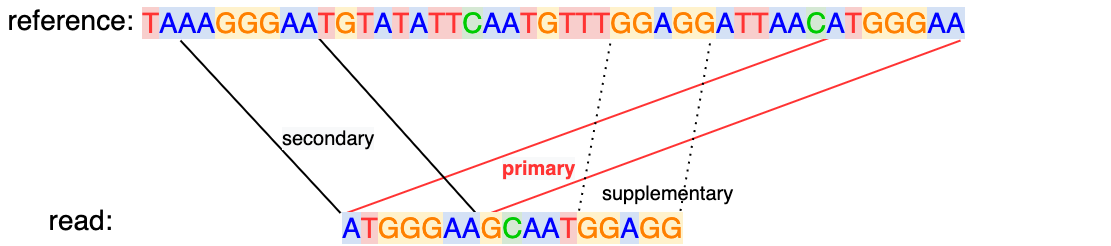
\includegraphics[width=1\columnwidth]{body/image/secondary-alignment.png}
\caption[secondary alignment]{BWA secondary alignment, supplementary alignment.}
\label{secondary-alignment}
\end{figure}

\begin{figure}[H]
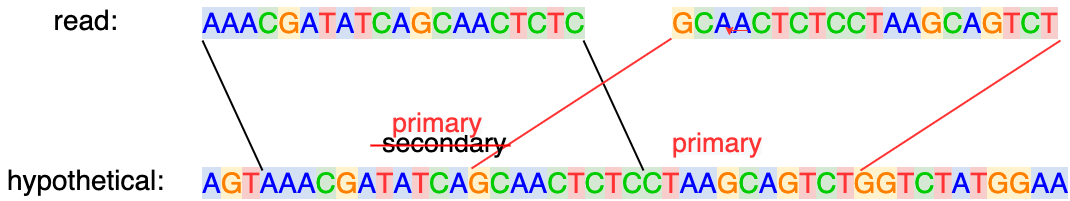
\includegraphics[width=1\columnwidth]{body/image/primary-alignment.png}
\caption[primary alignment]{The read index is used to find reads matching a hypothetical genome sequence.  BWA marks some matches as primary, etc., but we treat them all the same.}
\label{primary-alignment}
\end{figure}

Then we use BWA-MEM to search for our hypothetical sequence using seed alignment based on super maximal exact match, after this, we will get two sets of index as Figure \ref{read-index} shows, one set represents the start and end positions of the region on the hypothetical sequence, and the other set represents the index of the corresponding read region on the read-index. 

\begin{figure}[H]
\vspace{1em}
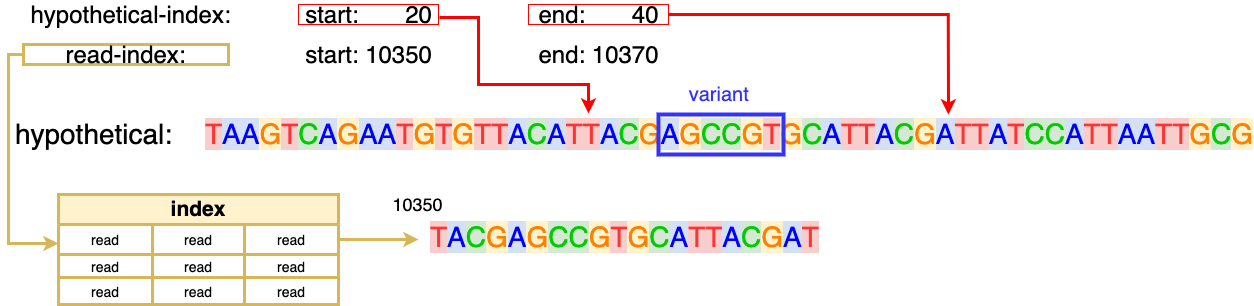
\includegraphics[width=1\columnwidth]{body/image/read-index.png}
\caption[read-index]{how to find matching read through read-index.}
\label{read-index}
\end{figure}

Through the index of hypothetical sequence, we can check whether it contains the variant, if not, we will filter it, as Figure \ref{filter-reads} shows.  At the end of this step, we can obtain a set of reads meeting our requirements, and then add them to the pileup.

\begin{figure}[H]
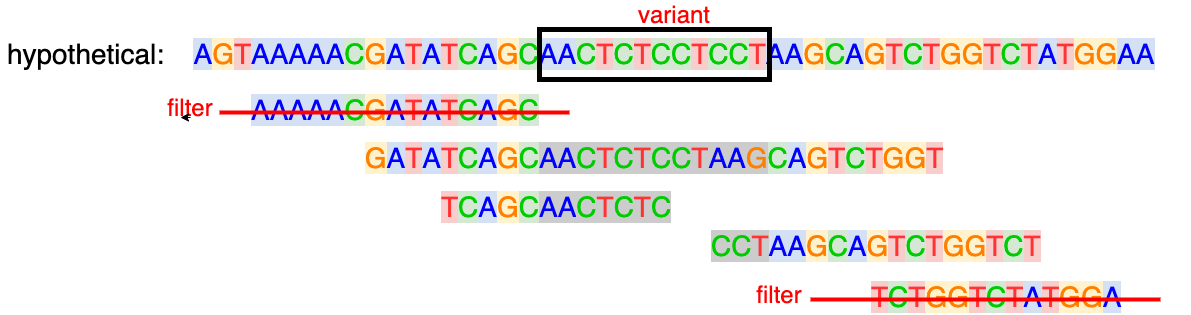
\includegraphics[width=1\columnwidth]{body/image/filter-reads.png}
\caption[Filter reads]{Filter reads that don't overlap the variant.}
\label{filter-reads}
\end{figure}

\section{Integrating new reads into the pileup}
In the last step, we need to compare all the read sets obtained in the previous step with the reads in the pileup. What is the pileup?
We start with a standard read mapping result stored in BAM file format.  We can observe that reads is mapped to a position in the reference genome. Many reads may align to the same region, and this ``pile'' of reads is called the pileup. Our final goal is to find reads that overlap with the same variant position but do not exist in the BAM file, (Figure \ref{exp-pileup} shows the pileup reads which overlap on a variant position.)

\begin{figure}[H]
\vspace*{1em}
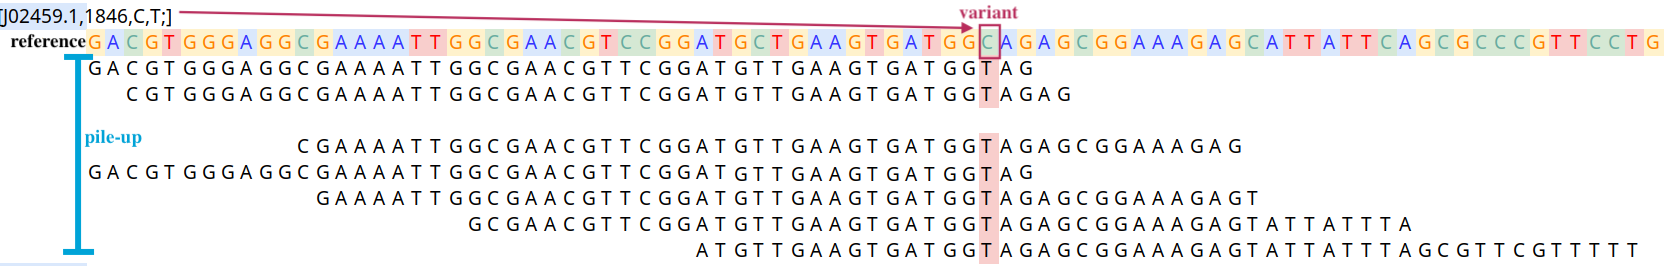
\includegraphics[width=1\columnwidth]{body/image/exp-pileup.png}
\caption[pileup]{pileup at the variant position.}
\label{exp-pileup}
\end{figure}

We can get the pileup from a BAM file quickly through the utility library \texttt{HTSlib}, and then compare the read set with these pileup reads, if the read does not exist in the pileup, it means that we have got the results we want.  The next step for our work is to convert this read, and use the two sets of index obtained in the previous step to generate some essential information that will be needed in our eagle calculation, including SAM flag and CIGAR string, SAM flag is represents the mapping status of this read and the CIGAR string encodes the detailed alignment of the read. We will explain how we get CIGAR string through two sets of indexes.

If we get the SAM flag and CIGAR directly through our two sets of indexes, what we get is the alignment information of hypothetical sequence mapping to read, like previous Figure \ref{read-index} shows, but what EAGLE needs is the alignment information of read mapping to reference sequence. So we need do some processing on the match positions.

First of all, from the position of matches to in read-index, we can directly obtain matching reads.  The other match position is relative to the start and end of our hypothetical sequence --- a length $2\ell$ sequence containing a candidate variant in the middle.  We need to convert positions in this sequence into positions in the reference genome to help us add the read to the pileup in such as way that EAGLE can consider it when evaluating that variant.

\noindent
This problem can be divided into 4 cases(Figure \ref{alignment-read}):
%%
\begin{enumerate}
\itemsep=-0.5em
\item the tail of read sequence overlaps with the variant.
\item the front of read sequence overlaps with the variant.
\item the center of read sequence overlaps with the variant.
\item all of read sequence overlaps with the variant.
\end{enumerate}


\begin{figure}[H]
\centering
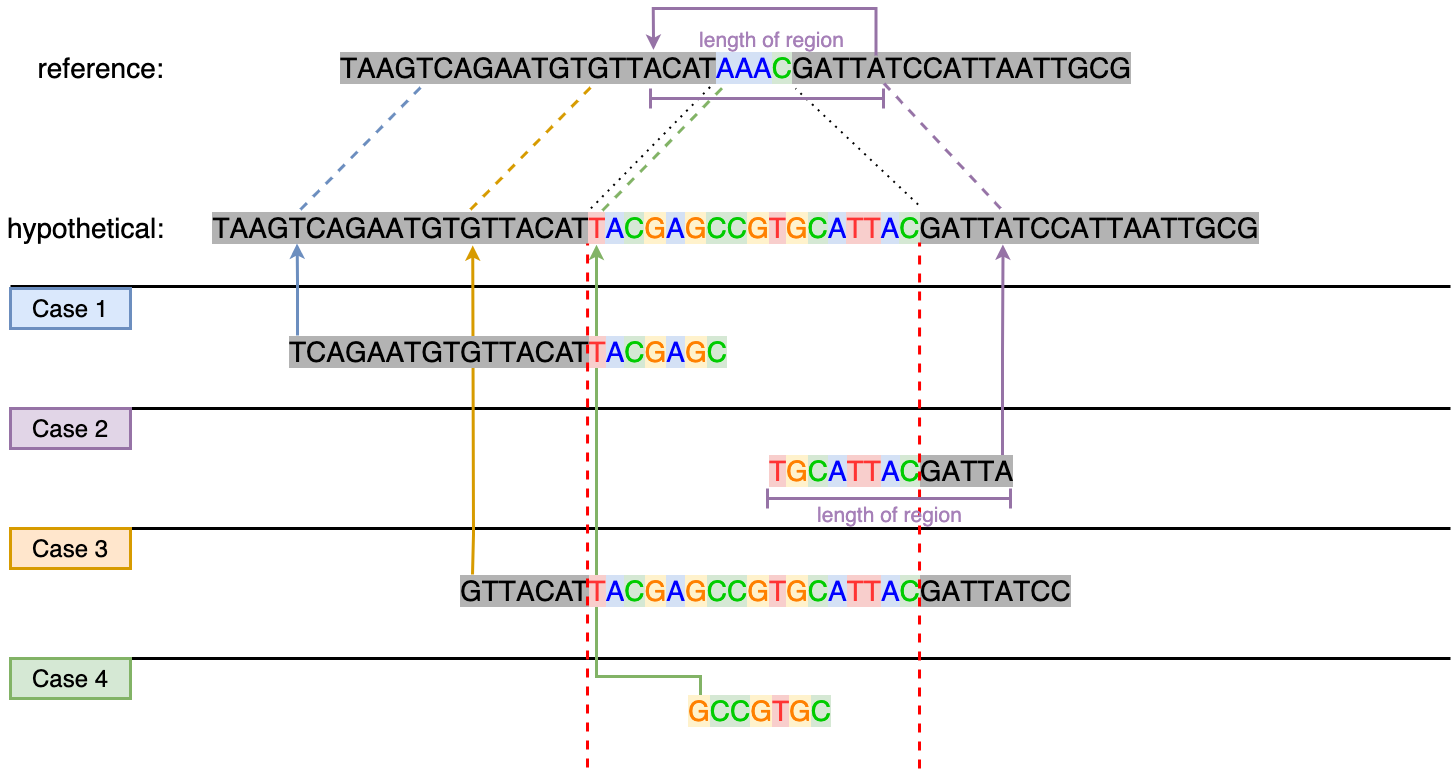
\includegraphics[width=1\columnwidth]{body/image/alignment-read.png}
\caption[alignment read]{Four cases related read to variant.  A read may overlap with part of a variant (left or right side), may completely include a variant, or be included by the variant.}
\label{alignment-read}
\end{figure}


For the first case and third case we can just directly get the reference position, and fourth case we use the position of variant.  In the second case, we need to use the end of the region to push-back the position.

In the last step, we already have read mapping position in the reference genome, so that we can create read alignment information. Most of them are nothing special and will not change as we change the alignment position, except for CIGAR string, we need to convert it from hypothetical sequence's alignment information mapped against read to the read's alignment information mapped against reference sequences (Figure \ref{convert-CIGAR}).  We use a small function we implemented to construct a CIGAR string for these reads.

\begin{figure}[H]
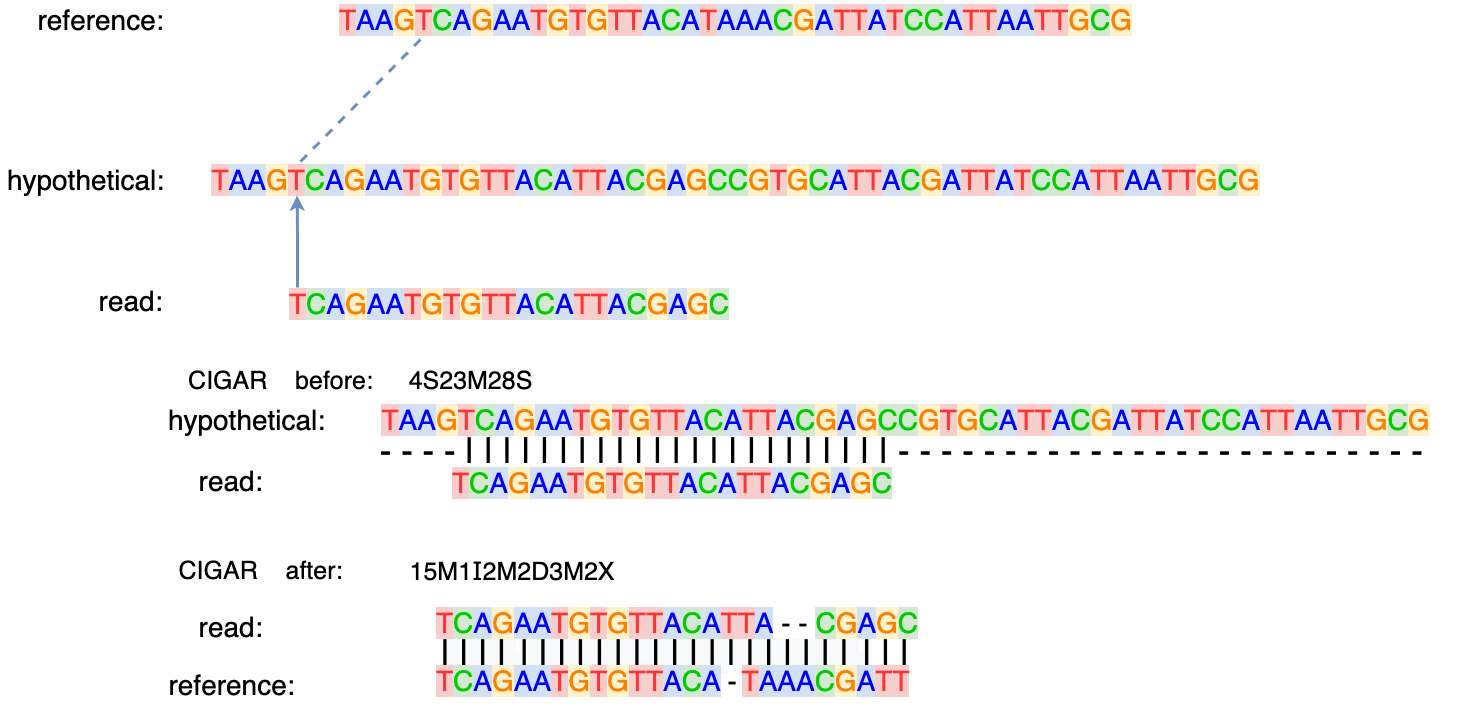
\includegraphics[width=1\columnwidth]{body/image/convert-CIGAR.png}
\caption[CIGAR strings]{How to convert CIGAR strings.}
\label{convert-CIGAR}
\end{figure}

Through these steps we can add read to the pileup for eagle to calculate likelihood.
